% ============================================================
%   CVE Text-Property-Graph example sub-graph
%   For: "Buffer overflow in OpenSSL 1.0.1f"
% ============================================================
%
% Standalone version of the "Example sub-graph" inset in
% model_architecture.tex (lines 141-161). Same nodes and edges,
% but laid out wide enough that the edge labels do not collide.
% Page sized close to the figure bounding box so
%   
\includegraphics[width=\linewidth]{CVE-graph-example}
% scales cleanly to a two-column figure width.
%
% Compile:
%   pdflatex -interaction=nonstopmode CVE-graph-example.tex
% ============================================================

\documentclass[10pt]{article}

\usepackage[paperwidth=180mm, paperheight=140mm, margin=4mm]{geometry}
\usepackage{tikz}
\usepackage{amsmath}
\usepackage{amssymb}
\pagestyle{empty}

\usetikzlibrary{positioning, arrows.meta, calc, fit, backgrounds}

% -- Colour palette (matches model_architecture.tex) --
\definecolor{nodeBase}{RGB}{ 70,130,180}
\definecolor{nodeSec}{RGB}{200, 80, 80}
\definecolor{edgeBase}{RGB}{ 60, 60, 60}
\definecolor{accent}{RGB}{ 20, 70,140}
\definecolor{frameFill}{RGB}{249,250,252}

\tikzset{
    bignode/.style={
        rounded corners=2pt, draw=nodeBase, fill=white,
        line width=0.45pt, inner sep=3pt,
        font=\scriptsize\sffamily, minimum height=5mm,
    },
    rootnode/.style={
        rounded corners=2pt, draw=accent, fill=white,
        line width=0.6pt, inner sep=3pt,
        font=\scriptsize\sffamily\bfseries, minimum height=5mm,
    },
    % Edge styles per relation type (each type gets its own
    % line style so a reader can tell them apart at a glance):
    %   lin       -> CONTAINS    (solid, dark grey)
    %   belongs   -> BELONGS_TO  (dotted, dark grey)
    %   nexttok   -> NEXT_TOKEN  (dotted, blue)
    lin/.style={
        -{Stealth[length=2mm]}, line width=0.5pt, draw=edgeBase,
    },
    belongs/.style={
        -{Stealth[length=2mm]}, line width=0.6pt, draw=edgeBase,
        dotted,
    },
    nexttok/.style={
        -{Stealth[length=2mm]}, line width=0.65pt, draw=nodeBase,
        dotted,
    },
    elab/.style={
        font=\tiny\sffamily, text=edgeBase,
        inner sep=1pt,
        fill=white, fill opacity=0.92, text opacity=1,
        rounded corners=1pt,
    },
    title/.style={
        font=\sffamily\bfseries\small, text=accent,
    },
    subtitle/.style={
        font=\sffamily\scriptsize, text=black!65,
    },
    legbox/.style={
        rectangle, rounded corners=1.5pt, draw=black!40, fill=white,
        line width=0.3pt, inner sep=3pt, font=\tiny\sffamily,
        align=left,
    },
}

\begin{document}

\noindent
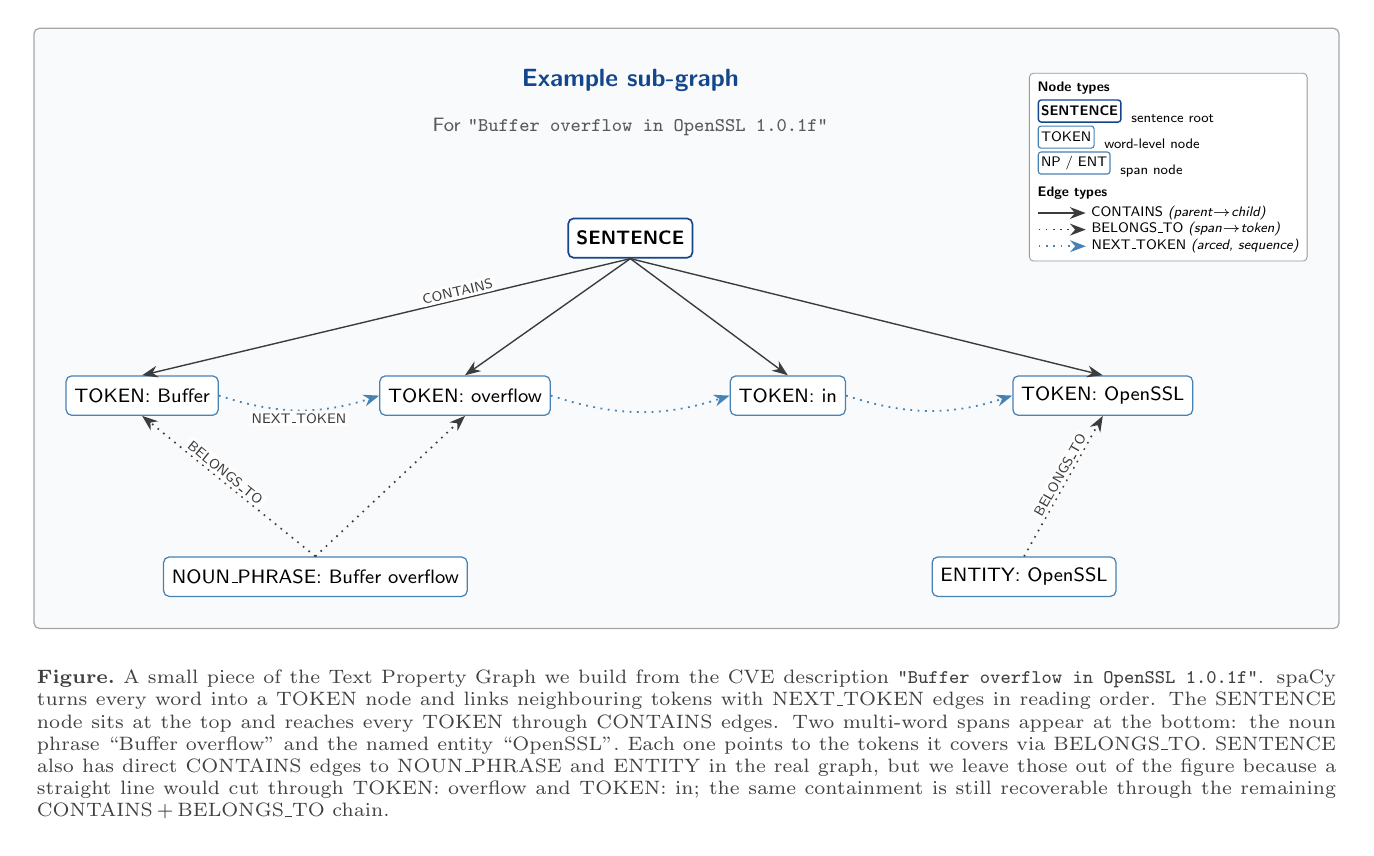
\begin{tikzpicture}

% ============================================================
%   Title block
% ============================================================
\node[title] (ttl) at (0, 5.6) {Example sub-graph};
\node[subtitle, below=0.8mm of ttl] (sub)
    {For \texttt{"Buffer overflow in OpenSSL 1.0.1f"}};

% ============================================================
%   Nodes
%   - SENTENCE root at top
%   - Four TOKEN nodes spaced widely on the middle row
%   - NOUN_PHRASE on the bottom-left, ENTITY on the bottom-right
% ============================================================
\node[rootnode] (S)  at ( 0.0,  3.6) {SENTENCE};

\node[bignode]  (T1) at (-6.2,  1.6) {TOKEN: Buffer};
\node[bignode]  (T2) at (-2.1,  1.6) {TOKEN: overflow};
\node[bignode]  (T3) at ( 2.0,  1.6) {TOKEN: in};
\node[bignode]  (T4) at ( 6.0,  1.6) {TOKEN: OpenSSL};

\node[bignode]  (NP) at (-4.0, -0.7) {NOUN\_PHRASE: Buffer overflow};
\node[bignode]  (E)  at ( 5.0, -0.7) {ENTITY: OpenSSL};

% ============================================================
%   Edges
%   Each edge type appears with its label on ONE representative
%   edge; sibling edges of the same type are drawn without labels
%   to keep the figure clean (the legend lists every type).
% ============================================================

% --- CONTAINS: SENTENCE -> {TOKEN x4} -----------------------
% Direct CONTAINS edges from SENTENCE to NOUN_PHRASE and ENTITY
% exist in the real graph as well, but they are omitted here:
% a straight S -> NP line would cross TOKEN: overflow and a
% straight S -> E line would cross TOKEN: in. The transitive
% containment (S contains TOKEN, TOKEN belongs to NP/ENTITY) is
% still visible through the remaining edges. The figure caption
% notes this omission.
\draw[lin] (S.south) --
    node[elab, pos=0.35, sloped, above=0pt] {CONTAINS} (T1.north);
\draw[lin] (S.south) -- (T2.north);
\draw[lin] (S.south) -- (T3.north);
\draw[lin] (S.south) -- (T4.north);

% --- BELONGS_TO: NP -> {T1, T2};  ENTITY -> T4 ---------------
\draw[belongs] (NP.north) --
    node[elab, pos=0.55, sloped, above=0pt] {BELONGS\_TO} (T1.south);
\draw[belongs] (NP.north) -- (T2.south);
\draw[belongs] (E.north)  --
    node[elab, pos=0.55, sloped, above=0pt] {BELONGS\_TO} (T4.south);

% --- NEXT_TOKEN: T1 -> T2 -> T3 -> T4 ------------------------
\draw[nexttok] (T1.east) to[bend right=18]
    node[elab, midway, below=0pt] {NEXT\_TOKEN} (T2.west);
\draw[nexttok] (T2.east) to[bend right=18] (T3.west);
\draw[nexttok] (T3.east) to[bend right=18] (T4.west);

% ============================================================
%   Legend (top-right): node and edge key
% ============================================================
\node[legbox, anchor=north east] (leg) at (8.6, 5.7) {
    \textbf{Node types}\\[1pt]
    \tikz{\node[draw=accent, fill=white, line width=0.5pt,
                rounded corners=1pt, font=\tiny\sffamily\bfseries,
                minimum height=2.8mm, inner sep=1pt] {SENTENCE};}\ \
        sentence root\\
    \tikz{\node[draw=nodeBase, fill=white, line width=0.4pt,
                rounded corners=1pt, font=\tiny\sffamily,
                minimum height=2.8mm, inner sep=1pt] {TOKEN};}\ \
        word-level node\\
    \tikz{\node[draw=nodeBase, fill=white, line width=0.4pt,
                rounded corners=1pt, font=\tiny\sffamily,
                minimum height=2.8mm, inner sep=1pt] {NP / ENT};}\ \
        span node\\[2pt]
    \textbf{Edge types}\\[1pt]
    \tikz[baseline=-0.5ex]{\draw[lin]     (0,0) -- (6mm,0);}\ CONTAINS\
        \textit{(parent$\to$child)}\\
    \tikz[baseline=-0.5ex]{\draw[belongs] (0,0) -- (6mm,0);}\ BELONGS\_TO\
        \textit{(span$\to$token)}\\
    \tikz[baseline=-0.5ex]{\draw[nexttok] (0,0) -- (6mm,0);}\ NEXT\_TOKEN\
        \textit{(arced, sequence)}
};

% ============================================================
%   Outer frame
% ============================================================
\begin{scope}[on background layer]
    \node[draw=black!35, line width=0.45pt, rounded corners=2pt,
          fill=frameFill,
          fit=(ttl)(sub)(S)(T1)(T4)(NP)(E)(leg),
          inner sep=4mm] (frame) {};
\end{scope}

% ============================================================
%   Caption (below the frame). Kept inside the standalone
%   bounding box so the figure is self-contained when viewed
%   on its own. When the figure is included in a paper via
%   \includegraphics{}, prefer the suggested \caption{...}
%   block reproduced as a comment at the end of this file.
% ============================================================
\node[font=\scriptsize, text=black!75, text width=165mm,
      align=justify, below=4mm of frame.south, anchor=north]
      (cap) {%
    \textbf{Figure.}\ A small piece of the Text Property Graph
    we build from the CVE description
    \texttt{"Buffer overflow in OpenSSL 1.0.1f"}. spaCy turns
    every word into a TOKEN node and links neighbouring tokens
    with NEXT\_TOKEN edges in reading order. The SENTENCE node
    sits at the top and reaches every TOKEN through CONTAINS
    edges. Two multi-word spans appear at the bottom: the noun
    phrase ``Buffer overflow'' and the named entity
    ``OpenSSL''. Each one points to the tokens it covers via
    BELONGS\_TO. SENTENCE also has direct CONTAINS edges to
    NOUN\_PHRASE and ENTITY in the real graph, but we leave
    those out of the figure because a straight line would
    cut through TOKEN: overflow and TOKEN: in; the same
    containment is still recoverable through the remaining
    CONTAINS$\,+\,$BELONGS\_TO chain.
};

\end{tikzpicture}

\end{document}

% ============================================================
%   Suggested LaTeX caption for paper integration
% ============================================================
%
% Copy this into a \begin{figure}...\end{figure} block:
%
% \begin{figure}[t]
%   \centering
%   
\includegraphics[width=\linewidth]{CVE-graph-example}
%   \caption{A small piece of the Text Property Graph we build
%   from the CVE description
%   \texttt{"Buffer overflow in OpenSSL 1.0.1f"}. spaCy turns
%   every word into a TOKEN node and links neighbouring tokens
%   with NEXT\_TOKEN edges in reading order. The SENTENCE node
%   sits at the top and reaches every TOKEN through CONTAINS
%   edges. Multi-word spans appear as NOUN\_PHRASE and ENTITY
%   nodes, each pointing to the tokens it covers via
%   BELONGS\_TO. SENTENCE also has direct CONTAINS edges into
%   NOUN\_PHRASE and ENTITY in the real graph; we leave those
%   out of the figure to keep the layout uncluttered.}
%   \label{fig:cve-graph-example}
% \end{figure}
%
% ============================================================
